\documentclass[12pt]{article}
\usepackage{calc}
\usepackage[usenames,dvipsnames]{xcolor}
\definecolor{lightgray}{gray}{0.9}

\usepackage{tikz}
\usetikzlibrary{calc}
\usepackage[graphics, tightpage, active]{preview}
\usepackage{amsmath}


\setlength{\PreviewBorder}{2pt}
\PreviewEnvironment{tikzpicture}

\usetikzlibrary{shapes,arrows}
\usetikzlibrary{calc, positioning}
\usepackage{pgfplots}
\usepackage{filecontents}

\usetikzlibrary{intersections}
\usepackage{tkz-euclide}
\usetkzobj{all}

%============================================================================================
%Additional commands
\tikzstyle{block} = [draw, rectangle, minimum height=2em, minimum width=4em]
%fill=blue!20
\tikzstyle{sum} = [draw, fill=blue!20, circle, node distance=1cm]
\tikzstyle{input} = [coordinate] \tikzstyle{output} = [coordinate]
\tikzstyle{pinstyle} = [pin edge={to-,thin,black}]

%============================================================================================
\begin{document}
%============================================================================================


%-----------------------------------------------------------------------------------------------------------------------------------------------------------------
 \def\radius{.7mm}
 \tikzstyle{branch}=[fill,shape=circle,minimum size=3pt]

\tikzstyle{dotted}= [dash pattern=on .01mm off 2.5mm,
                                         line cap=round]
                                         
% Radius for arc over intersection
\def\radius{1.mm} 

 \begin{tikzpicture}[auto, node distance=2cm,>=latex']

    \node[block] (system) at (6, -2) {Server};
    \node[output] at (7.3, -2) (sys_output) {};
    \node[sum, left of=system] (sum)  at (4, -2) {};
    \node[above left = of sum, anchor=west, align = left] at (1,-1) (block1) {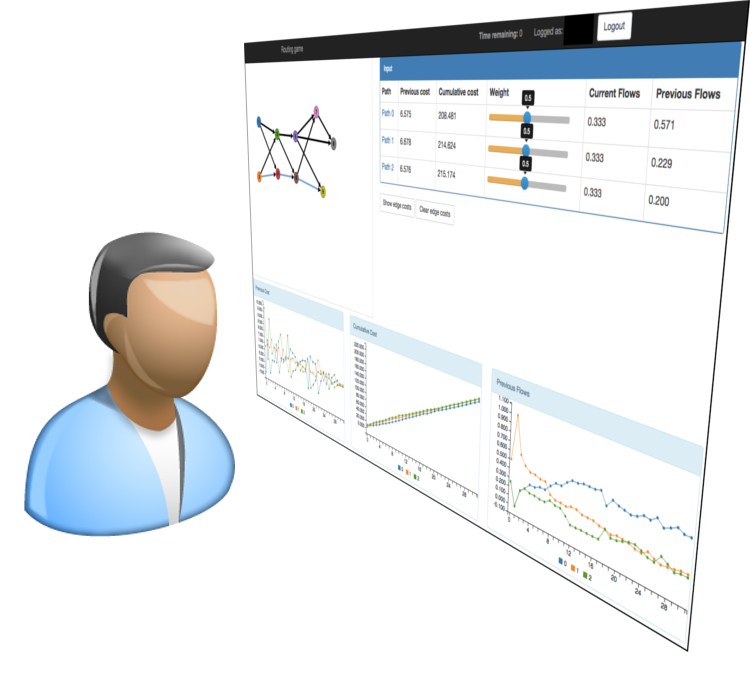
\includegraphics[width=.08\textwidth]{user_interface_perspective2}};
    \node[left = of sum, anchor=west, align = left] at (1.6,-2) (block2) {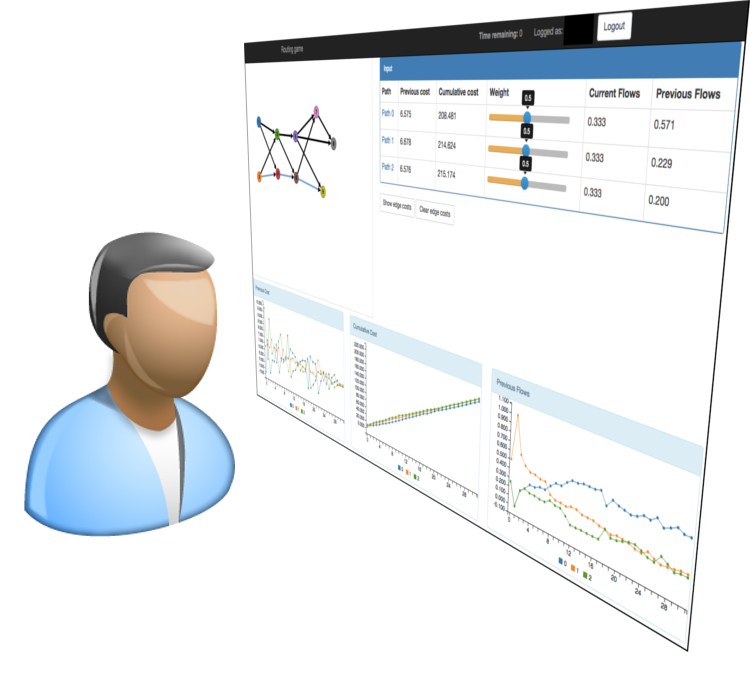
\includegraphics[width=.08\textwidth]{user_interface_perspective2}};
    \node[below left = of sum, anchor=west, align = left] at (1,-3) (block3) {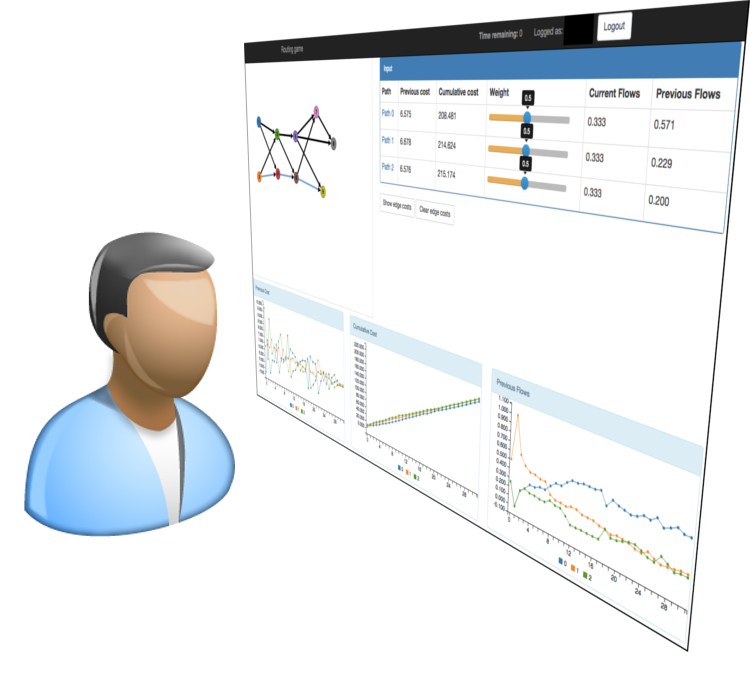
\includegraphics[width=.08\textwidth]{user_interface_perspective2}};

   \coordinate[below = 0.3cm of block1] (b1_turn);
   \coordinate[above = 0.3cm of block2] (b2_turn);
   \coordinate[above = 0.3cm of block3] (b3_turn);
   \coordinate(system_b1_turn) at (3.7, 1.55);
   \coordinate(system_b2_turn) at (3.7, -0.85);
   \coordinate(system_b3_turn) at (3.7, -3.265);

   \draw[->] (sum) -- node {$\bar x^{(t)}$} (system);
   \draw[-] (system) -- (sys_output);

   \draw[->, name path = line one_to_sum] (block1.east) -| node [near start] {$\bar x_1^{(t)} $} (sum) ;
   \draw[->] (sys_output) |- (system_b1_turn) -| node [near start, above right = 0.0cm and 1.5cm of block1] {$(\bar \ell_{1}^{(t)}, \bar \ell^{(t-1)}_{1}, \dots)$} (block1.north);

   \draw[->] (block2) |- node [near end]  {$\bar x_2^{(t)} $} (sum);
   \path[name path = line output_to_two] (sys_output) |- (system_b2_turn) -| (block2.north);

   \draw[->, name path = line three_to_sum] (block3) -| node [near start] {$\bar x_3^{(t)} $}  (sum);
   \path[name path = line output_to_three] (sys_output) |- (system_b3_turn) -| (block3.north);
   
  \path [name intersections={of = line one_to_sum and line output_to_two}];
  \coordinate (S)  at (intersection-1);
  
   \path[name path=circle] (S) circle(\radius);
  
  \path [name intersections={of = circle and line output_to_two}];
  
  \coordinate (I1)  at (intersection-1);
  \coordinate (I2)  at (intersection-2);
    
    \tkzDrawArc[color=black](S,I1)(I2);
    
    \draw[-, name path = line output_to_two] (sys_output) |- (system_b2_turn) -- node [near start, above right = 0.0cm and 0.0cm of block1] {$(\bar \ell_{2}^{(t)}, \bar \ell_2^{(t-1)}, \dots)$}  (I1);
    \draw[->] (I2) -| (block2.north);

  \path [name intersections={of = line three_to_sum and line output_to_three}];
  \coordinate (S1)  at (intersection-1);
  
   \path[name path=circle1] (S1) circle(\radius);
  
  \path [name intersections={of = circle1 and line output_to_three}];
  
  \coordinate (I3)  at (intersection-1);
  \coordinate (I4)  at (intersection-2);
  
      \tkzDrawArc[color=black](S1,I3)(I4);

   \draw[-] (sys_output) |- (system_b3_turn) -| node [near start, above right = 0.0cm and 0.0cm of block1] {$(\bar \ell_{3}^{(t)}, \bar \ell_3^{(t-1)}, \dots)$}  (I3);
   
       \draw[->] (I4) -| (block3.north);

	\draw[dotted,line width = 2mm] (0.3,-5.2) -- (0.3, -5.9);

  \end{tikzpicture}

%-----------------------------------------------------------------------------------------------------------------------------------------------------------------




\end{document}